\section{Introduction}
% 在大数据的时代,人们越来越依赖于数据分析进行决策。例如,当一家超市想要合理进货以便最大化其利润时,他需要考虑超市历史的售卖订单、市场上客户对于商品的喜爱度、各类商品的利润率等方面,这往往需要通过分析各个方面大量的数据来做决定。
In the era of big data, people increasingly rely on data analysis for decision-making~\cite{albright2020business}. 
% For instance, when a supermarket aims to optimize its profits through informed inventory management, it needs to consider various factors, such as historical sales orders, customer preferences, profit margins for different items. This often necessitates the analysis of a vast amount of data from various aspects to make informed decisions.
% 为了完成数据分析任务,那些没有服务器的人通常把数据分析的任务托管到云服务器上。但在使用云服务器进行数据分析的同时,人们会担心这些重要的数据遭到泄漏,因为这个数据往往涉及到个人的隐私、商业机密等。
To perform data analysis, individuals without their own servers typically delegate data analysis tasks to cloud servers~\cite{sandhu2021big}. However, while using cloud servers for data analysis, there are concerns about the potential leakage of this critical data~\cite{purohit2013data}, as it often involves personal privacy or business secrets.
% 为了避免数据的泄漏的问题,越来越多的相关技术被提出以解决数据泄露的问题。这些技术包括:多方安全计算、同态加密、联邦学习、可信执行环境等。
To address the issue of data leakage, an increasing number of relevant technologies have been proposed. These technologies encompass: Secure Multi-Party Computation (MPC)~\cite{lindell2020secure,patra2021aby2,dalskov2022fast}, Homomorphic Encryption (HE)~\cite{marcolla2022survey,lu2021pegasus,bossuat2021efficient}, Federated Learning (FL)~\cite{li2021survey,bonawitz2017practical,shayan2020biscotti}, Trusted Execution Environments (TEE)~\cite{zheng2021survey,tsai2017graphene,priebe2018enclavedb}.
% 在这些技术中,MPC和HE具备极高的安全性,因为它是密码学安全的,但由于MPC和HE包含了复杂的密码学操作,其性能相较于其他几类技术表现极差。FL常见于机器学习的场景,主要用于联合建模,对于一般的数据分析场景并不适用。TEE满足各类通用计算的场景,其计算性能较高,但其基于硬件的安全性,相较于MPC和HE的密码学安全,其安全性更低,而且经常出现新发现的基于TEE的侧信道攻击。
Among these technologies, TEE is versatile, catering to a wide range of general computing scenarios and offers higher computational performance.
% Among these technologies, MPC and HE provide exceptionally high security as they are based on cryptographic security principles. However, due to the complexity of cryptographic operations involved, they exhibit significantly lower performance~\cite{alaya2020homomorphic,evans2018pragmatic} compared to other categories. FL is commonly encountered in machine learning scenarios, primarily for collaborative modeling~\cite{li2021survey}, and may not be well-suited for typical data analysis settings. TEE is versatile, catering to a wide range of general computing scenarios and offers higher computational performance. Nevertheless, its security, based on hardware, is lower compared to the cryptographic security of MPC and HE, and it is susceptible to newly discovered side-channel attacks~\cite{nilsson2020survey}.

% 然而,随着数据分析的场景越来越复杂,现有的这些技术不能直接应用于那些复杂的场景,来解决数据泄漏的问题。
However, with the growing complexity of data analysis scenarios involving multiple roles, existing technologies are not readily applicable to effectively address data leakage in these intricate contexts.
% 现有的数据分析场景中,仅存在租户和云计算服务提供商两个角色,现有技术主要是为了防止云计算服务提供商泄漏租户的数据。但是现在的数据分析场景中,包含了数据提供方、数据使用方、模型提供方、云计算服务提供商这些角色,数据需要防止被数据提供方之外的所有角色泄漏。除此之外,还需要维护数据分析场景中各方的权益,例如,数据使用方得到合理的分析结果,数据提供方、模型提供方、云计算服务提供商获得相应的收益。
% 通过图更形象地描述场景的复杂?
In existing data analysis scenarios, there are only two roles, as shown in Figure~\ref{fig:analysis_scenarios}(a): tenants and cloud service providers. Existing technologies primarily focus on preventing cloud service providers from leaking tenant data. However, in today's data analysis scenarios, there are multiple roles involved, as shown in Figure~\ref{fig:analysis_scenarios}(b), including data providers, data users, model providers, and cloud service providers. Data must be protected from leakage by all parties outside of the data provider. In addition to this, it is necessary to safeguard the interests of all parties involved in the data analysis scenario. For instance, data users should obtain fair and valid analysis results, while data providers, model providers, and cloud service providers should engage in equitable revenue sharing.

% 因此,在针对复杂的数据分析场景时,我们需要检测数据使用方是否通过输出的计算结果中包含敏感信息以泄漏数据,模型提供方是否通过恶意的模型泄漏数据,云计算服务提供商通过篡改hypervisor、操作系统、内存、磁盘等泄漏数据,数据提供方、模型提供方以及云计算服务提供商共同生成的计算结果是否合法。
Therefore, when dealing with data analysis scenarios with multiple roles, we need to detect whether data users attempt to leak data by extracting sensitive information from the computed results, whether model providers engage in data leakage through malicious models, whether cloud service providers attempt data leakage by manipulating hypervisors, operating systems, memory, disks, and other means, and whether the computed results generated collectively by data providers, model providers, and cloud service providers are legitimate.

% 很多相关的研究被提出,来解决复杂的数据分析场景时所面临的问题,包括SDTE,PrivacyGuard等。
Many relevant studies have been proposed to address the challenges faced in data analysis scenarios with multiple roles, including SDTE~\cite{dai2019sdte}, PrivacyGuard~\cite{xiao2020privacyguard}, SPDS~\cite{wang2020spds}, Amanuensis~\cite{hardin2022amanuensis} and etc.
SDTE~\cite{dai2019sdte} introduced an innovative model known as ``data processing-as-a-service'' in the data trading industry. Leveraging this model, it achieves secure data trading through a series of trading protocols.
PrivacyGuard~\cite{xiao2020privacyguard} utilizes smart contracts to define data usage policies and leverages TEE for efficient contract execution while safeguarding private data.
SPDS~\cite{wang2020spds}, much like PrivacyGuard, employs smart contracts to define data usage policies and implements a two-phase delivery protocol to ensure secure release of computing results and payment.
Amanuensis~\cite{hardin2022amanuensis} explores the intersection of blockchain technology and TEE to address the challenges of data provenance, confidentiality, and user privacy in data sharing.

\begin{figure}[t]
  \centering
{
\begin{tabular}{cc}
      \subfloat[tenant and cloud service provider]{
  \hspace*{-0.7cm}
        \scalebox{0.42}{
        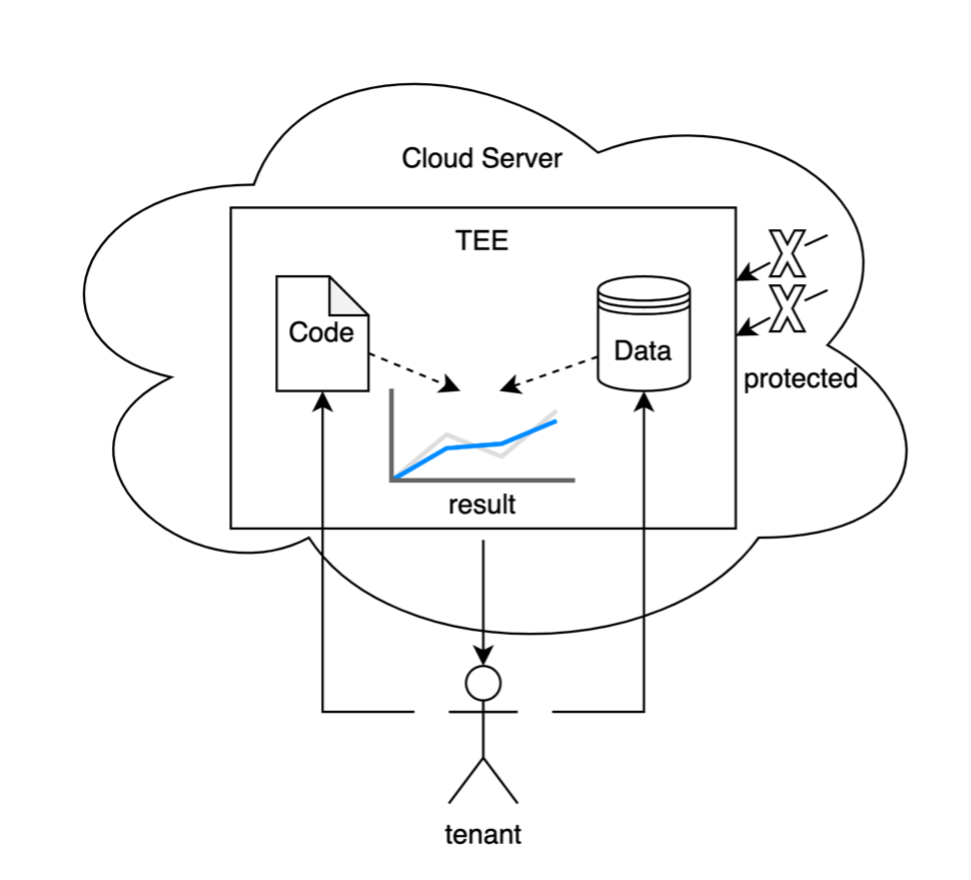
\includegraphics{images/analysis_2_roles.png}
        }
      } &
      \subfloat[multiple roles]{
  \hspace*{-1cm}
        \scalebox{0.42}{
        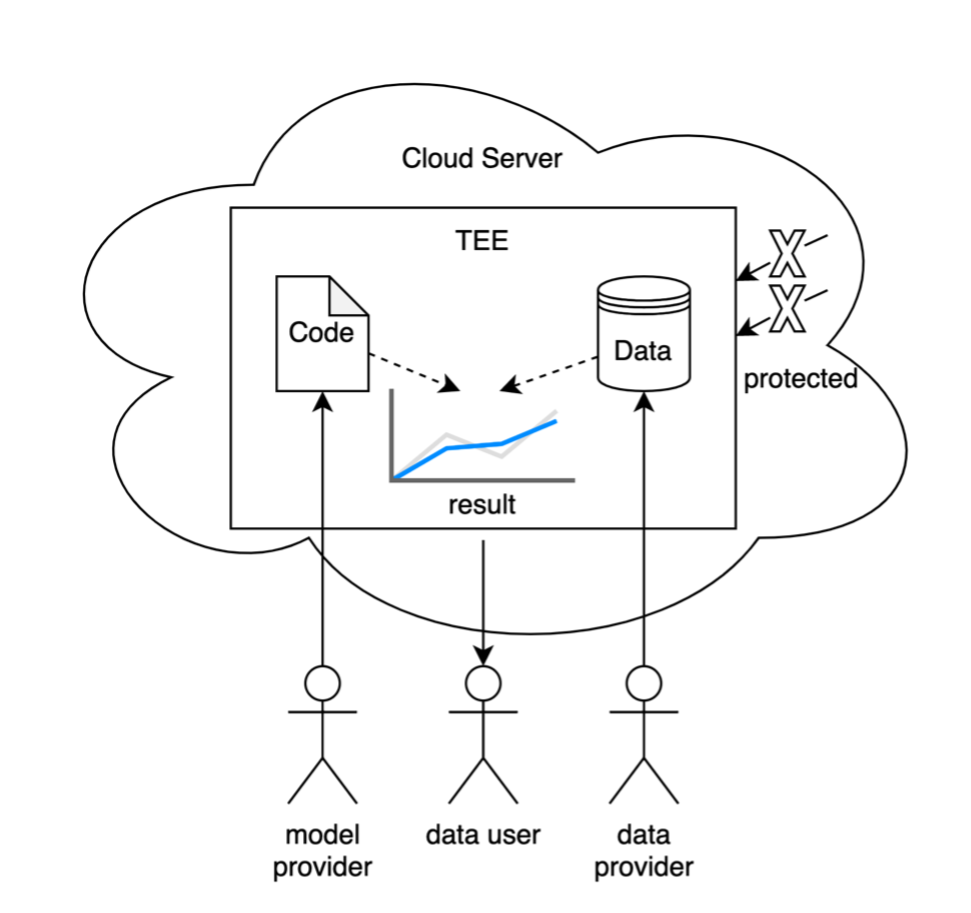
\includegraphics{images/analysis_4_roles.png}
        }
      }    \\
\end{tabular}
  }
  \caption{\small Data Analysis Scenarios with Two Roles vs. Multiple Roles.}
  \label{fig:analysis_scenarios}
\end{figure}
% 然而,这些相关的研究在解决复杂的数据分析场景时,仍存在一些限制。
However, these relevant studies still exhibit certain limitations when addressing these data analysis scenarios. 
% 首先,这些相关的研究工作不能保证数据分析结果中不会泄漏数据。虽然这些工作引入了数据使用规则,用以描述哪些人以什么样的价格访问哪些类型的数据,但对数据进行分析的程序是存在作恶的可能的,分析程序的最终输出结果可能是包含敏感信息泄漏的。一个最简单的例子是,分析程序直接输出原始数据,这样数据分析结果就获取到了完整的原始数据。
First, these related research efforts do not guarantee the prevention of data leakage within data analysis results. Although these works introduce data usage policies to describe who can access what kinds of data at what price, there is the possibility of malicious behavior in data analysis programs. The final output of the analysis program may include the leakage of sensitive information. An example is when the analysis program directly outputs the raw data, allowing the data analysis results to gain access to the complete, raw data.
% 一个straghtforward的解决方案是,要求分析程序公开,数据提供方可以审核分析程序是否存在泄漏数据的代码。但是对于模型提供方而言,模型也是他们重要的资产,他们不希望模型公开。另一方面,对于复杂的分析程序来说,审核分析程序存在巨大的工作量,不可能要求每一个分析任务都去进行审核,这会大大降低数据分析的效率。
A straightforward solution is to require the analysis program to be open and accessible for data providers to audit, ensuring that it does not contain code that could lead to data leaks. However, for model providers, their models are valuable assets, and they may be reluctant to make them publicly available. On the other hand, auditing complex analysis programs represents a significant workload, and it is not feasible to require audits for every analysis task, as this would significantly reduce the efficiency of data analysis.

% 结果可验证
% 其次,当前的工作中并不能保证计算结果的可信与可验证。具体来说,数据使用方得到计算结果后,他不能确定这个计算结果确实是通过指定的数据与指定的模型运行之后得到的计算结果,而不是一个随机生成的结果。更进一步,数据使用方并没有任何方式去验证这个结果的正确性。如果计算结果的可信和可验证都无法保证,那么完全可以用一个伪造的计算结果来欺骗数据使用方,数据使用方的利益将会受到损害。
Second, the existing works cannot ensure the trustworthiness and verifiability of computation results. Specifically, when a data user receives computation results, they are unable to confirm that these results indeed stem from running the specified data through the specified model and are not simply randomly generated. Furthermore, data users lack any means to validate the correctness of these results. Without the assurance of both trustworthiness and verifiability of the computation results, there is the potential for deceptive results to be used to mislead data users, jeopardizing their interests.

% 分析程序一致性
% 最后,当前的工作中每一次进行数据分析任务都需要使用remote attestation来保证分析程序的一致性,但是有相关工作表明,remote attestation具有低效、依赖可信第三方的缺点。
Finally, in existing works, remote attestation is required for every data analysis task to ensure the consistency of the analysis program. However, related works~\cite{chen2019opera,chen2022mage} have shown that remote attestation has drawbacks such as inefficiency and dependence on trusted third parties.
% 以Intel SGX中的Enhanced Privacy ID(EPID)为例,一次remote attestation的过程会涉及到Intel Provisioning Service(IPS)、Intel Attestation(IAS) Service、Intel-signed provisioning enclave(PvE)、Intel-signed quoting enclave(QE)以及分析程序Enclave之间的交互。这些服务和Enclaves之间的交互需要通过广域网传输数据,同时,传输的数据需要加密保证其安全性,对于频繁的数据分析任务而言,性能上会有较大的损失。另一方面,IPS和IAS是Intel提供的中心化服务,remote attestation需要依赖其稳定运行。
Taking Intel Software Guard Extensions (SGX) Enhanced Privacy ID (EPID) as an example, a single remote attestation process involves interactions between the Intel Provisioning Service (IPS), Intel Attestation Service (IAS), Intel-signed provisioning enclave (PvE), Intel-signed quoting enclave (QE), and the analysis program enclave. These interactions require data transmission over a wide area network, and the transmitted data must be encrypted to ensure its security. For frequent data analysis tasks, this can lead to significant performance overhead. On the other hand, IPS and IAS are centralized services provided by Intel, making remote attestation dependent on their stable working.

In this paper, we propose Fidelius, a system that leverages Intel SGX and blockchain to enhance data analysis security, addressing the previously mentioned limitations.
% 其中,Intel SGX保证数据分析过程的security和integrity,区块链用于可信的传输、存储和验证。
Intel SGX ensures the security and integrity of the data analysis process, while the blockchain is utilized for trustworthy transmission, storage, and verification.

% 为了解决计算结果泄漏数据的问题,Fidelius使用了静态二进制分析的方法,检查模型提供方的分析程序是否遵循隐私描述语言。其中,我们引入的隐私描述语言将数据的运算规则描述为有限状态机,反映了从输入数据到输出数据的状态转换,不在隐私描述语言描述的状态转换,都会被认为违反了隐私规则。
To address the issue of data leakage in computation results, Fidelius employs a static binary analysis approach~\cite{schulte2019gtirb} to examine whether the analysis program provided by the model adheres to a privacy description language (PDL). In this context, the introduced PDL characterizes the computational rules of data as a finite state machine (FSM), capturing the state transitions from input data to output data. Any state transitions not described in the PDL are considered as violations of the privacy rules.

% 为了解决计算结果的可信与可验证的问题,Fidelius提供了一套密码协议,该协议中由数据使用方提供一个私钥,该私钥通过加密转发至分析程序的Enclave中,并签名计算结果。由于该私钥仅在指定的分析程序Enclave中解密获得,数据提供方、模型提供方、云计算服务提供商均无法获取,故只要被签名的计算结果能够通过验证,说明计算结果确实出自指定的分析程序且可验证。
To ensure the trustworthiness and verifiability of computation results, Fidelius offers a cryptographic protocol. In this protocol, the data user provides a private key, which is securely transmitted to the analysis program's Enclave and used to sign the computation results. Since this private key can only be decrypted within the specified analysis program's Enclave, it remains inaccessible to the data provider, model provider, and cloud service provider. Therefore, if the signed computation results can be successfully verified, it confirms that the results indeed originate from the specified analysis program and are verifiable.

% 为了解决remote attestation低效、持续依赖中心化服务的问题,Fidelius结合设计的密码协议以及local attestation实现分析程序的一致性验证。Fidelius设计了密钥管理的Enclave,在初始化的过程中获取密钥的授权,在此后的所有数据分析任务中,使用该经授权的密钥执行local attestation完成分析程序的一致性验证。
To address the issues of the inefficiency and continued reliance on centralized services in remote attestation, Fidelius combines a designed cryptographic protocol with local attestation to achieve the consistency verification of analysis programs. Fidelius introduces a Key Management Enclave that obtains authorized keys during initialization. Subsequently, in all data analysis tasks, this authorized key is used to perform local attestation, ensuring the consistency of the analysis program.

The main contributions of this paper are summarized as follows.
\begin{itemize}
    \item First, we introduce the Privacy Description Language (PDL) combined with static binary analysis to rigorously enforce data confidentiality and prevent sensitive data leakage in computation outcomes.
    \item Second, we design a cryptographic protocol to ensure the trustworthiness and verifiability of computation results.
    \item we integrate the cryptographic protocol with a local attestation mechanism to ensure the integrity and correctness of analysis programs executed within protected environments.
    \item Finally, we evaluate the performance of Fidelius, and the experimental results demonstrate that it incurs minimal overhead, contributing less than 2\% to the data analysis system, while surpassing existing solutions by more than 30 times.
\end{itemize}



